\documentclass[UTF8,12pt]{article}
\usepackage[utf8]{inputenc}
\usepackage[T1]{fontenc}
\usepackage{vmargin} % page format
\usepackage{soul}       % underline multiple lines
\usepackage{enumerate}
\usepackage{enumitem}
\usepackage{color}
\usepackage{amsmath}
\usepackage{multirow}
\usepackage{amssymb}
\usepackage{bbm}
\usepackage{graphicx}
\usepackage{subfig}
\usepackage{diagbox}
\usepackage[pdfstartview=FitH,
CJKbookmarks=true,
bookmarksnumbered=true,
bookmarksopen=true,
colorlinks=true,                        
linkcolor=black]{hyperref}
\usepackage[numbers]{natbib}
\newcommand{\sinc}{\mathrm{sinc}}
\setpapersize{USletter}
\setmarginsrb{1 in}{1 in}{1 in}{0.5 in}{0pt}{0mm}{0pt}{0.5 in}
\pagestyle{empty}
\pagestyle{plain}
\setlength{\parskip}{1em}
\renewcommand{\baselinestretch}{1.5}
\usepackage{sectsty}% section font size
\usepackage{titlesec}% section spacing
\sectionfont{\fontsize{12}{0}\selectfont}
\subsectionfont{\fontsize{12}{0}\selectfont}
\titlespacing\section{0pt}{12pt plus 4pt minus 2pt}{0pt plus 2pt minus 2pt}
\titlespacing\subsection{0pt}{12pt plus 4pt minus 2pt}{0pt plus 2pt minus 2pt}
\titlespacing\subsubsection{0pt}{12pt plus 4pt minus 2pt}{0pt plus 2pt minus 2pt}

\title{Predicting Hand-written Digits using Backpropagation}
\date{2019\\ April}
\author{Yue WU\\ yw9998\\CS 391L}
\begin{document}
	\maketitle
	\section{Introduction}
	This homework aims at implementing the backpropagation algorithm to detect hand-written digits automatically. We will use a certain amount (ntrain) of training images included in a training set of 60000 images to derive an algorithm that can detect the digits shown in a test set of 10000 images. Each image contains 784 pixels.
	\section{Methods}
	For each image, values for the pixels are stored in a matrix named $X (ntrain - 784)$, and the numbers of the group that each image belongs to are stored in a vector named $Y$. The numbers from $"0"$ to $"9"$ stored in $Y$ are called "labels". Figure \ref{fig:1_visualization} shows some of the handwritten digits. In this homework, we mapped $"0"$ to $"10"$ in order to make things more compatible with MATLAB indexing where there is no zero index. We then expanded the $Y$ vector to a matrix $ry$ containing only $0$s and $1$s, where the position of $1$s indicates the index:
	\begin{equation}
		ry = \begin{bmatrix}
			0 & 0 & 1 & 0 & 0 & 0 & 0 & 0 & 0 & 0\\ 
			0 & 1 & 0 & 0 & 0 & 0 & 0 & 0 & 0 & 0\\ 
			... & ... & ... & ... & ... & ... & ... & ... & ... & ...\\ 
			0 & 0 & 0 & 0 & 0 & 1 & 0 & 0 & 0 & 0
		\end{bmatrix}
	\end{equation}
	\begin{figure}[!ht]
		\centering
		\subfloat[]{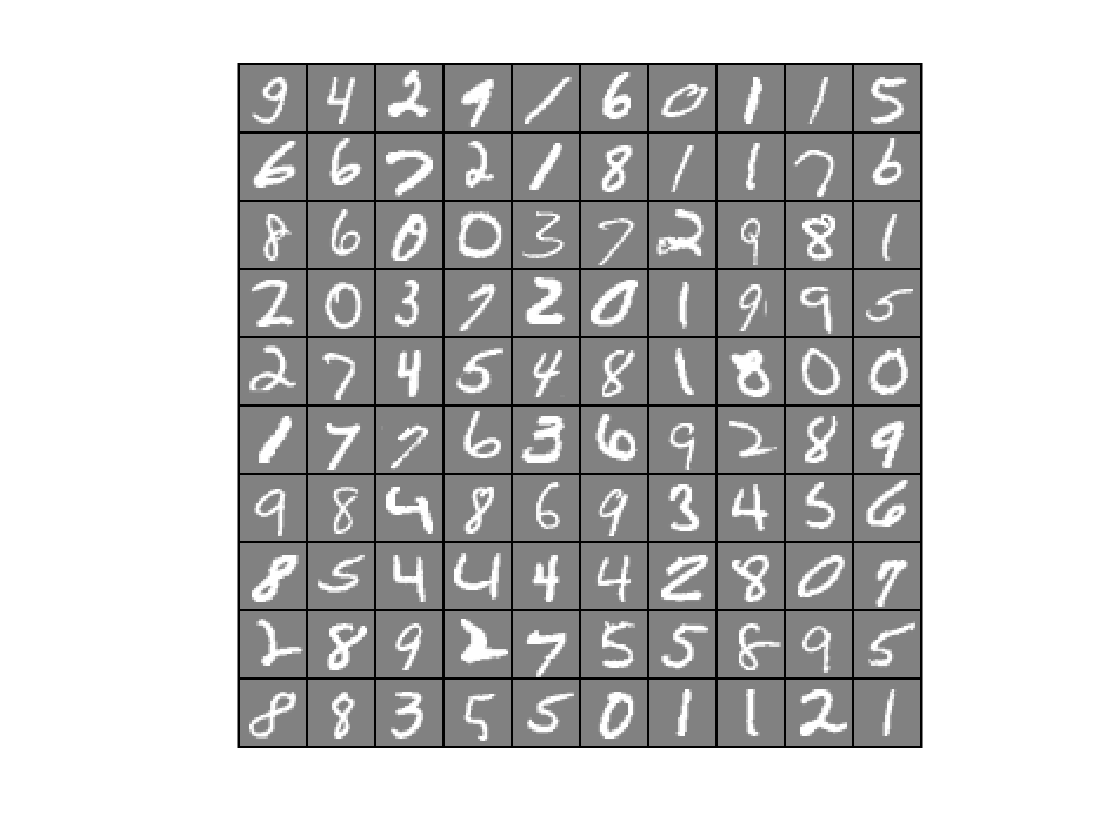
\includegraphics[width=0.75\linewidth]{figures/1_visualization.png}}
		\caption{\label{fig:1_visualization}Handwritten digits.}
	\end{figure}
	
	When applying backpropagation (Figure \ref{fig:2_NN}), we first set the parameters ($\Theta$s) in the model to some random small values. Then we do feedforward and calculate the cost and gradient for the neural network. We can check if the learning process is converging by checking if the cost is generally decreasing after each iteration, and we can update values for the parameters with the cost and gradient for each parameter that we just calculated. We will explain the procedures in detail in the following paragraph, and we will use a model with one input layer, two hidden layers, and one output layer as an example.
	\begin{figure}[!ht]
		\centering
		\subfloat[]{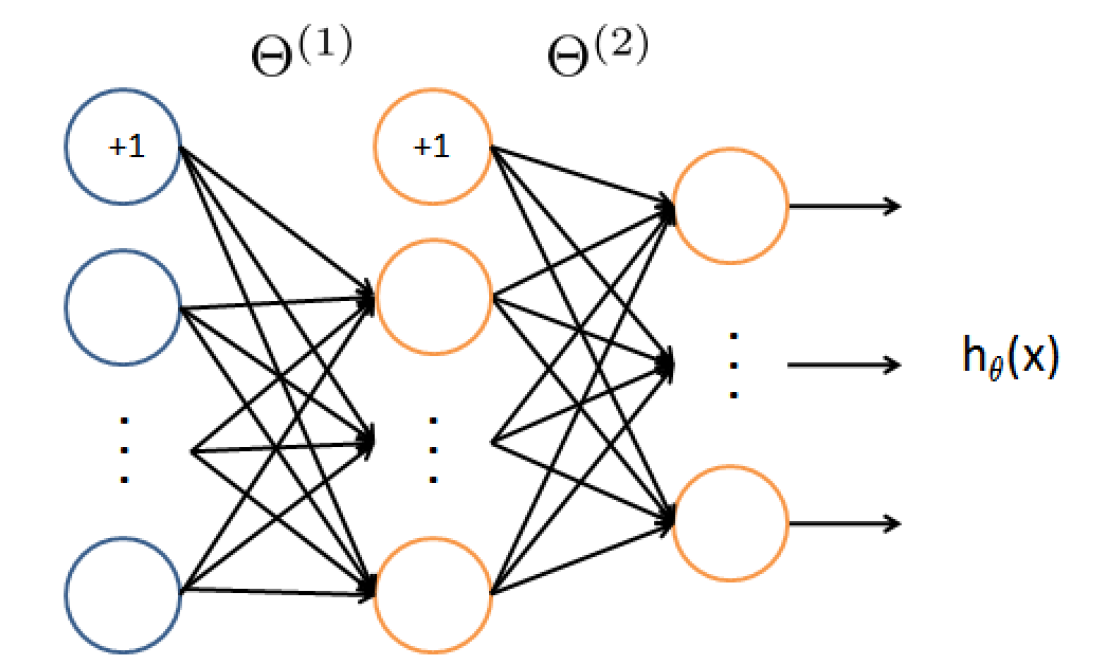
\includegraphics[width=0.75\linewidth]{figures/2_NN.png}}
		\caption{\label{fig:2_NN}Neural network model.}
	\end{figure}
	In this homework, we first initialize the parameters $\Theta^{(1)}$, $\Theta^{(2)}$, and $\Theta^{(3)}$ to be some random small values. Then, we do feedforward to calculate the predicted $Y$ values using the following equations:
	\begin{align}
	a^{(1)} &= X\\
	z^{(2)} &= a^{(1)}\Theta^{(1)}{'}\\a^{(2)} &= actfunction(z^{(2)})\\
	z^{(3)} &= a^{(2)}\Theta^{(2)}{'}\\a^{(3)} &= actfunction(z^{(3)})\\
	z^{(4)} &= a^{(3)}\Theta^{(3)}{'}\\a^{(4)} &= sigmoid(z^{(3)})
	\end{align}
	where,
	\begin{equation}
	sigmoid(z^{(3)})=\frac{1}{1+e^{-z^{(3)}}}
	\end{equation}
	the $a^{(4)}$ showing here is the prediction we calculated using the current parameters and training samples. The "actfunction" shown here is the activation function of our choice. We will compare the performance of four activation functions: sigmoid, tanh, ReLU and SeLU. Next, we compare $a^{(4)}$ with $ry$ and compute the costs. We applied two different loss functions to compute the cost: the cross entropy loss (log loss) function (Equation \ref{eq:crossentropy}) and the hinge loss function (Equation \ref{eq:hingeloss}).
	\begin{equation}
	\label{eq:crossentropy}
	\mathcal{L}  = -ry*log(a^{(4)})-(1-ry)*log(1-a^{(4)})
	\end{equation}
	\begin{equation}
	\label{eq:hingeloss}
	\mathcal{L}  = max(0,1-ry*a^{(4)})
	\end{equation}
	Then, the regularized cost can be calculated by:
	\begin{align}
	J(\theta) = \frac{1}{ntrain}\sum_{i=1}^{ntrain}\sum_{k=1}^{K}\left [ -y_{k}^{(i)}log((h_{\theta}(x^{(i)}))_{k})-(1-y_{k}^{(i)})log(1-(h_{\theta}(x^{(i)}))_{k}) \right ]\nonumber\\+\frac{\lambda}{2*ntrain}\left [ \sum_{j=1}^{nfirst}\sum_{k=1}^{ninput}(\Theta_{j,k}^{(1)})^{2}+\sum_{j=1}^{nsecond}\sum_{k=1}^{nfirst}(\Theta_{j,k}^{(2)})^{2} +\sum_{j=1}^{noutput}\sum_{k=1}^{nsecond}(\Theta_{j,k}^{(3)})^{2}\right ]
	\end{align}
	where $ntrain$ is the number of training samples, $ninput$ is the number of input parameters (which equals to 784 in this case), $nfirst$ is the number of parameters in the first layer, $nsecond$ is the number of parameters in the second layer, and $noutput$ is the number of output parameters (which equals to 10 in this case).
	
	Now we have the cost, which is a value to determine how far away our prediction is from the actual value. We still need the gradients for each parameter to update the parameters and improve the model using stochastic gradient descent (SGD). The gradient is calculated using the following series of equations:
	\begin{align}
	(Cross \ Entropy) \ \delta^{(4)} &= a^{(4)}-ry\\(Hinge \ Loss) \ \delta^{(4)} &= -ry*a^{(4)}*(1-a^{(4)})\\
	\delta^{(3)}&=\delta^{(4)}*\Theta^{(3)}*actfuncgrad(z^{(3)})\\
	\delta^{(2)}&=\delta^{(3)}*\Theta^{(2)}*actfuncgrad(z^{(2)})\\
	\Delta^{(3)} &= \delta^{(4)}{'}*a^{(3)}\\
	\Delta^{(2)} &= \delta^{(3)}{'}*a^{(2)}\\
	\Delta^{(1)} &= \delta^{(2)}{'}*a^{(1)}
	\end{align}
	Then, the gradients are:
	\begin{equation}
	\frac{\partial }{\partial \Theta_{ij}^{(l)}}J(\Theta) = \frac{1}{m}\Delta_{ij}^{(l)}+\frac{\lambda}{m}\Theta_{ij}^{(l)}
	\end{equation}
	We update the parameters using:
	\begin{equation}
	\Theta^{(l)} = \Theta^{(l)}-\alpha\frac{\partial \mathcal{L} }{\Theta^{(l)}}
	\end{equation}
	where $\alpha$ is the learning rate.
	
	The updated parameters are then put back into the model and calculate new predictions, costs, and gradients until the cost finally reaches a pre-set threshold.

	\section{Results}
	\subsection{Comparing loss functions}
	In this experiment, we used a model with two hidden layers to explore the difference in performance between two categorical loss functions: cross entropy loss function (Equation \ref{eq:crossentropy}) and hinge loss function (Equation \ref{eq:hingeloss}). The input layer contains 784 units, the first hidden layer contains 50 units, the second hidden layer contains 30 units, and the output layer contains 10 units which represent the ten labels. We used the sigmoid activation function, and we set the threshold for the cost to be 0.1, the learning rate $\alpha$ to be 0.1. To accelerate the procedure, we applied mini-batch gradient descent and set the size of the batches to 200. We set the regularization parameter $\lambda$ to be 0 (no regularization). The results are shown in the following form:
	\begin{figure}[!ht]
		\centering
		\subfloat[]{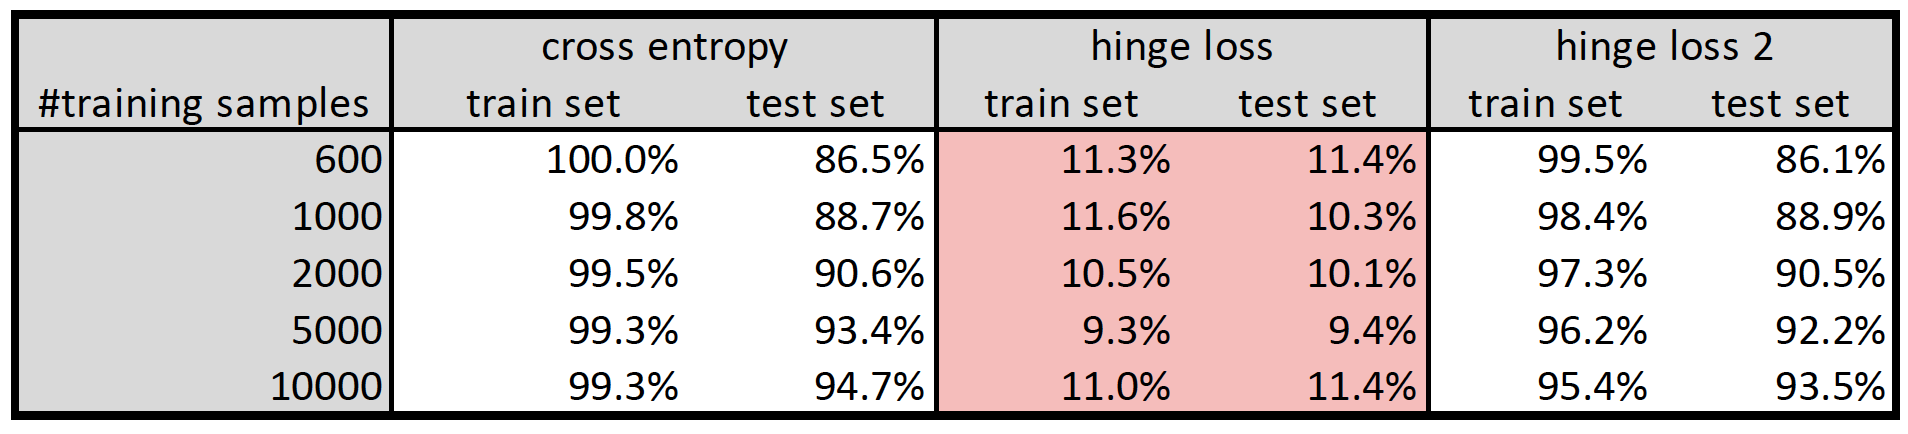
\includegraphics[width=1\linewidth]{figures/lossfunc.png}}
		\caption{\label{fig:lossfunc}Accuracies of prediction when applying two categorical loss functions: cross entropy loss function and hinge loss function.}
	\end{figure}
	
	The two columns under "cross entropy" shows prediction accuracies for both training set and testing set for different numbers of training samples using cross entropy loss function. The two columns under "hinge loss" shows results obtained when applying hinge loss function in both calculations of cost and of gradients. The two columns under "hinge loss 2" shows results when the hinge loss function is used only when applying cost, and we still used the cross entropy loss function when calculating gradients. 
	
	Our experiment shows that hinge loss uses much fewer iterations for the cost to reach the threshold, however, the accuracies are very low, or in other words, all predictions failed and the training was failed. This is because hinge loss found out that simply predicting all "1"s can help it reach the threshold easily, which causes problems when calculating the gradients. This is not the case for cross entropy because predicting all "1"s will make the cost become infinity. Therefore, when we used the cross entropy loss function to calculate the gradients while keep using hinge loss function to check the cost, we can still arrive at pretty good results. Besides, training set accuracy is becoming lower as the number of training samples increases, because the number of units is not enough to "overfit" all data, while testing set accuracy increases as the number of training samples increases.
	\subsection{Comparing activation functions}
	Next, we used the same model as before, fixed the loss function to be cross entropy loss function, and compare the performance between four different activation functions: sigmoid, tanh, ReLU and SeLU (Equation \ref{eq:actfunc1} - Equation \ref{eq:actfunc2}). Results are shown in the form:
	\begin{figure}[!ht]
		\centering
		\subfloat[]{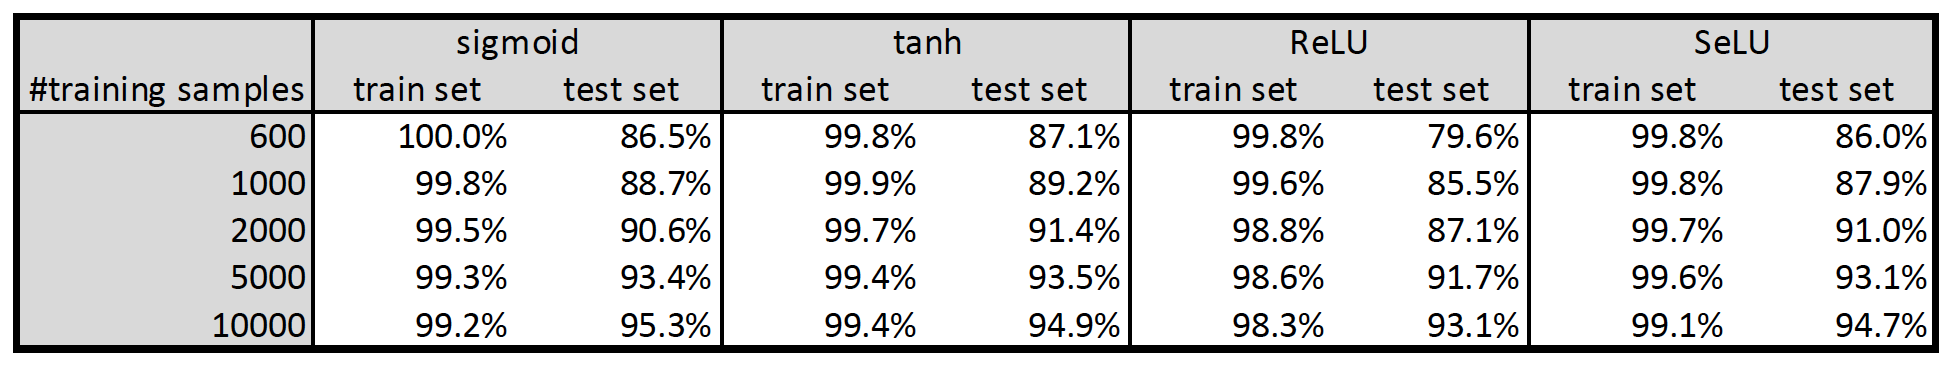
\includegraphics[width=1\linewidth]{figures/actfunc.png}}
		\caption{\label{fig:actfunc}Accuracies of prediction when applying four activation functions: sigmoid, tanh, ReLU and SeLU.}
	\end{figure}
	\begin{align}
	\label{eq:actfunc1}
	(sigmoid) \ \ \ \ g(z) &= \frac{1}{1+e^{-z}}\\
	(tanh) \ \ \ \ g(z) &= \frac{e^{z}-e^{-z}}{x^{z}+x^{-z}}\\
	(ReLU) \ \ \ \ g(z) &= max(z,0)\\
	\label{eq:actfunc2}
	(SeLU) \ \ \ \ g(z) &= \lambda\left\{\begin{matrix}
	x \ \ \ \ \ \ \ \ \ \ \ \ \ \ if \ x> 0\\
	\alpha e^{x}-\alpha \ \ \ \ \ \ if \ x\leq 0
	\end{matrix}\right.
	\end{align}
	
	Similar to before, training set accuracy is becoming lower as the number of training samples increases, because the number of units is not enough to "overfit" all data. And testing set accuracy increases as the number of training samples increases. Sigmoid, tanh, and SeLU have similar performance. ReLU is also good but the accuracy is slightly lower than the other three, although it requires fewer iterations and reaches the threshold faster. A potential problem with backpropagation is called "vanishing gradients". When the gradients are close to zero, the weights will not adjust and the whole process stops. ReLU was designed to overcome the problem because as long as the value is larger than zero, the gradient will be 1. However, a potential problem with ReLU is that when the changes in weights are high, the resulting value in the next iteration will be small, leading to the activation function stuck at the left side of the $y$-axis, where the gradient is zero. This is called "dying ReLU". This might be the reason for the low accuracy for ReLU in our experiment. On the other hand, SeLU, which is very similar to ReLU at the right side of the $y$-axis, is able to overcome the problem of "dying ReLU" while still has a low possibility of experiencing "vanishing gradients" because of internal normalization.
	\subsection{Comparing depth and width}
	Then, applying a similar model with the categorical loss function fixed to be cross entropy loss function and the activation function fixed to be sigmoid, we tried different numbers of depth (hidden layers) and width (units in each hidden layer) for $1000$ training samples. The results are shown below:
	\begin{figure}[!ht]
		\centering
		\subfloat[]{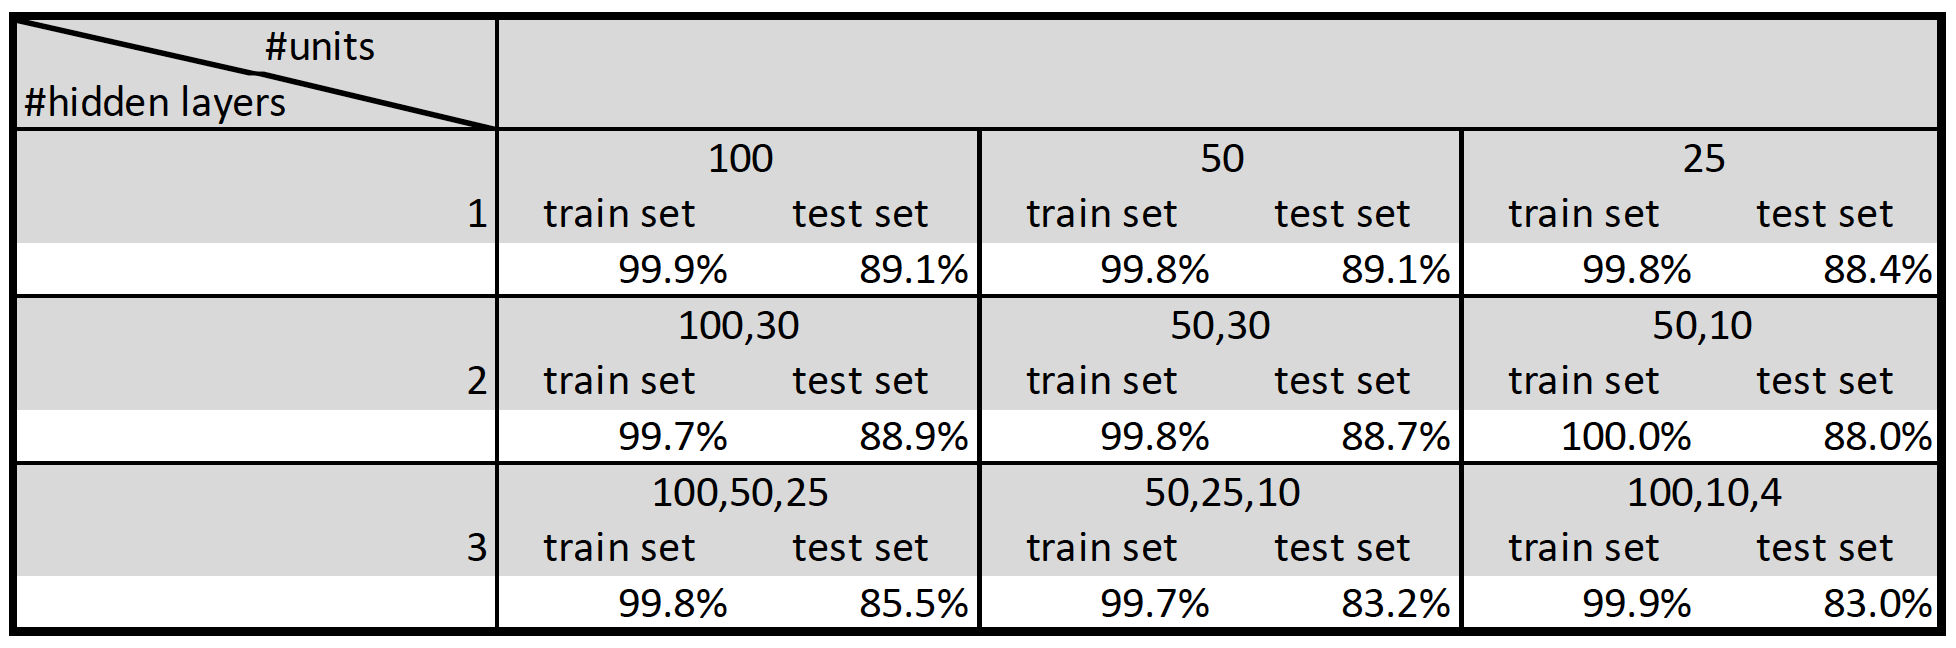
\includegraphics[width=1\linewidth]{figures/model.png}}
		\caption{\label{fig:model}Accuracies of prediction when using different numbers of layers and units.}
	\end{figure}
	
	We have "$4$" as the smallest number of units here because "$4$" is the least amount of units required to separate $10$ categories. However, this makes it requires much more iterations than other cases to reach the threshold and produce an acceptable prediction result, and the accuracy is still lower than the other two. We also found out that more units in each layer give higher testing set accuracy, while more layers do not necessarily lead to higher testing set accuracy, as the possibility of overfitting also increases as the number of layers increases. Therefore, selecting appropriate numbers of layers and units is important to achieving satisfying results.
	
	\section{Conclusion}
	In this homework, we have shown that for categorical loss functions, the cross entropy loss function is more suitable than hinge loss function in our case, as hinge loss tends to simply predict all "1"s so that it can reach the threshold easily, which causes problems when calculating the gradients. For activation functions, Sigmoid, tanh, and SeLU have similar performance. ReLU is also good but the accuracy is slightly lower than the other three. ReLU can overcome the problem of "vanishing gradients", and SeLU can deal with both "vanishing gradients" and "dying ReLU". Besides, Training set accuracy is becoming lower as the number of training samples increases because the number of units is not enough to "overfit" all data. While testing set accuracy increases as the number of training samples increases. We also found out that more units in each layer give higher testing set accuracy, while more layers do not necessarily lead to higher testing set accuracy. Therefore, it is important to select appropriate numbers of layers and units in order to achieve satisfying results.
	
\end{document}